\section{Robot Operating System 2 (ROS 2)}
\label{sec:ros2}

Robot Operating System (ROS) \citep{cit:quigley2009} merupakan sebuah \emph{robotics middleware} bersifat \emph{open source} yang digunakan untuk membantu pengembangan sistem yang ada pada robot.
Fitur utama yang ada pada ROS adalah desain sistem dimana data yang diterima maupun dikirim ke setiap komponen yang ada pada robot dilakukan secara terabstraksi dengan adanya \emph{hardware abstraction}.
Dengan adanya hal tersebut,
	algoritma yang ada pada suatu program dapat digunakan pada robot yang berbeda,
	terlepas dari perbedaan perangkat yang ada di setiap robot.

Untuk memungkinkan adanya \emph{hardware abstraction},
	ROS menggunakan \emph{graph architecture} yang memungkinkan suatu \emph{node} untuk berkomunikasi dengan \emph{node} lain melalui sebuah \emph{topic} yang sama.
Pada ROS, \emph{hardware abstraction} tersebut terbentuk dengan menggunakan \emph{topic} yang memiliki nama dan struktur data yang sama yang merepresentasikan jenis komponen yang dimiliki suatu robot.
Nantinya, Setiap node yang ada dapat menerima maupun mengirimkan data melalui \emph{topic} tersebut,
	terlepas dari bagaimana maupun darimana data yang dikirimkan tersebut berasal.

Pada ROS terdapat berbagai macam \emph{tools} yang sudah tersedia untuk membantu pengembangan sistem yang ada pada robot seperti \emph{command line} yang membantu dalam \emph{debugging} program,
	konfigurasi parameter secara dinamis,
	\emph{monitoring} robot secara visual, dan lain sebagainya.
Selain itu, dengan \emph{package management} yang ada pada ROS,
	setiap orang bisa menggunakan \emph{package} yang sudah ada maupun menambahkan \emph{package} baru untuk mempermudah pengembangan lebih lanjut dari suatu robot,
	tanpa perlu membuat ulang keseluruhan sistem yang dibutuhkan.

Generasi kedua dari Robot Operating System, ROS 2,
	merupakan kelanjutan dari ROS yang mengusung reliabilitas dan performa untuk penggunaan \emph{real-time} pada robot sembari masih mendukung fitur yang dimiliki oleh ROS sebelumnya \citep{cit:maruyama2016}.
Berbeda dengan pendahulunya yang menggunakan TCPROS/UDPROS sebagai sistem komunikasi yang digunakan di setiap node,
	ROS 2 menggunakan \emph{Data Distribution Service} (DDS) \citep{cit:castellote2003} \citep{cit:schlesselman2004}, standar industri untuk sistem komunikasi \emph{real-time} dan \emph{end-to-end middleware}.
Dengan penggunaan DDS tersebut, ROS 2 akan lebih terfokus pada penggunaan \emph{middleware} di bidang robotika,
	sedangkan komunikasi tingkat rendah yang dilakukan diantara setiap \emph{node} akan dikembalikan kepada implementasi DDS yang digunakan.

% \begin{figure}[ht]
%   \centering
% 	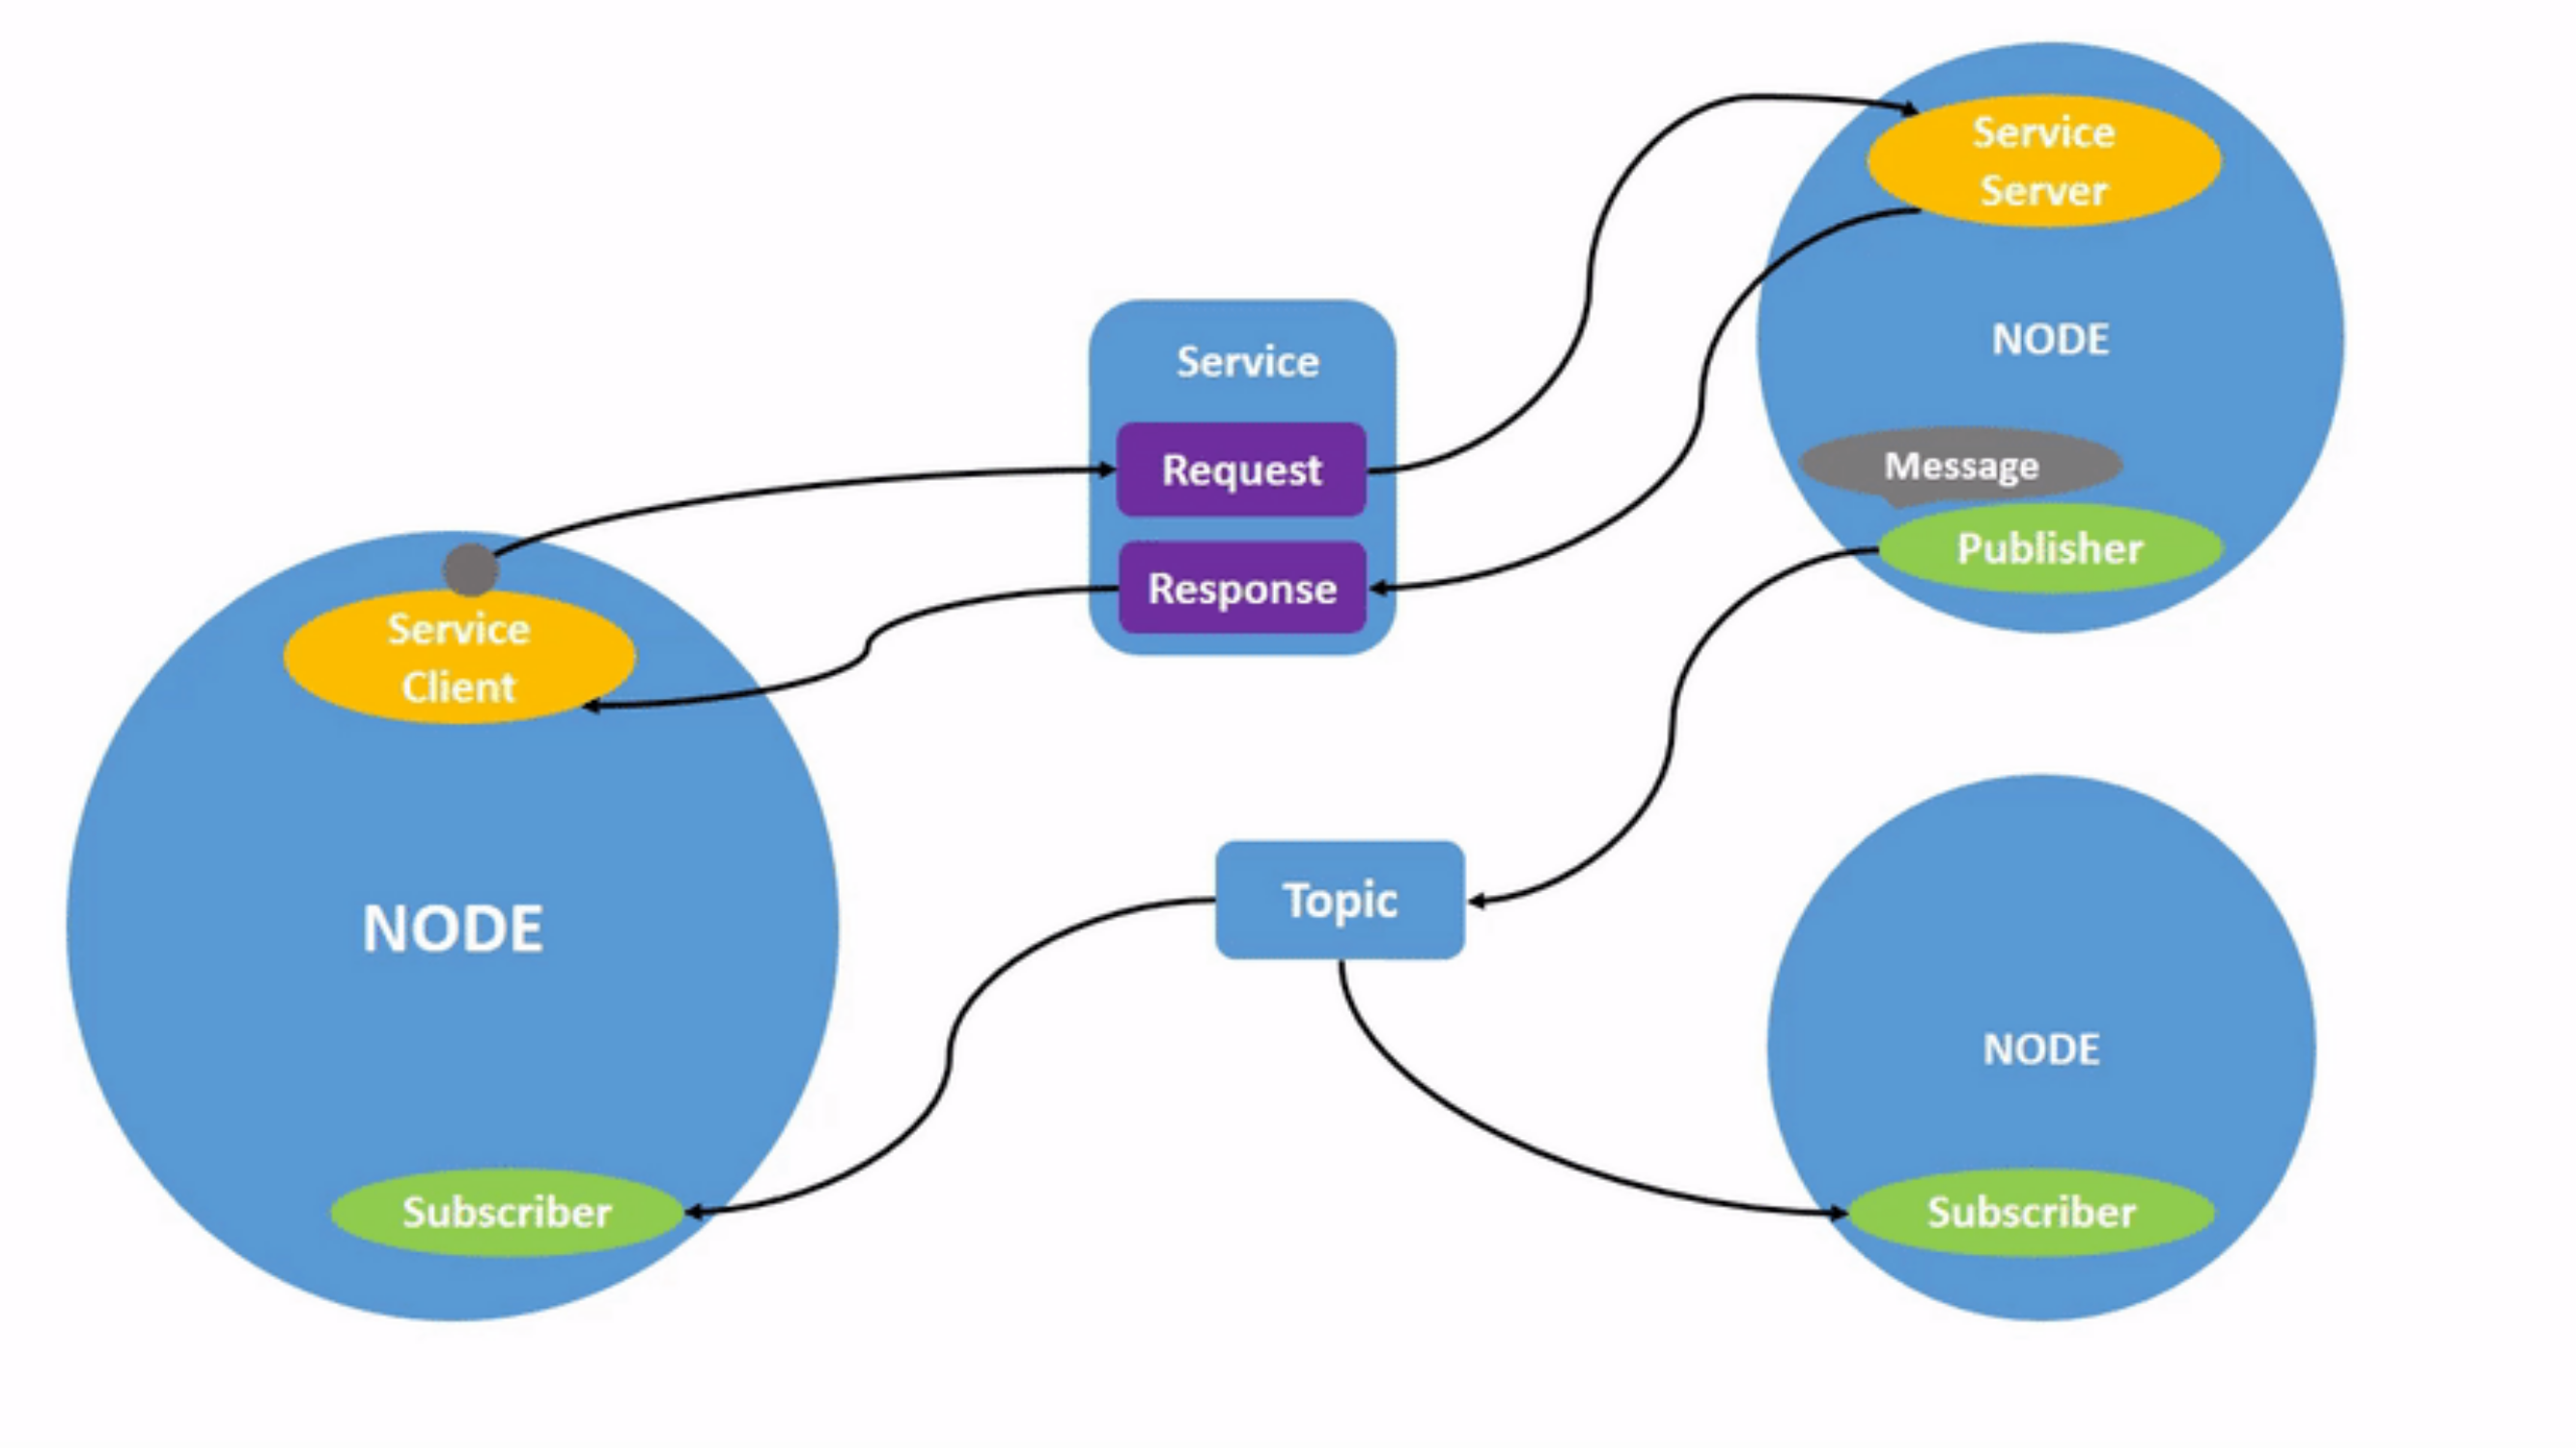
\includegraphics[scale=0.4]{gambar/komunikasi-ros.png}
% 	\caption{Diagram komunikasi antar node pada ROS 2 \citep{url:ros2nodes}.}
% 	\label{fig:komunikasiros}
% \end{figure}

\subimport{2-ros2}{1-rmw.tex}
\subimport{2-ros2}{2-rcl.tex}
% \subimport{2-ros2}{3-ros2-node.tex}
% \subimport{2-ros2}{4-ros2-topic.tex}
% \subimport{2-ros2}{5-ros2-service.tex}
% \subimport{2-ros2}{6-ros2-cli.tex}
% \subimport{2-ros2}{7-rqt.tex}
% \subimport{2-ros2}{8-rviz2.tex}
